% Skills routing diagram — companion to Figure 1 (architecture) in dsagt.tex.
% Standalone so it exports straight to latex/skills-routing.png:
%   pdflatex skills-routing.tex
%   pdftoppm -png -r 175 -singlefile skills-routing.pdf skills-routing
%
% Colour semantics (see legend): blue = external (skill repos, agent),
% green = DSAgt service (SkillRouter), orange = DSAgt store / skill (Skills
% Catalog, Skill Directory, the bundled skill-creator).  Concern bands are
% uniform faint outlines.  SkillRouter is the single skill-MCP entry point:
% every skill tool is labelled on the router operation it drives.
\documentclass[border=2mm]{standalone}
\usepackage{tikz}
\usepackage{lmodern}
\usetikzlibrary{positioning, arrows.meta, fit, backgrounds, calc}

\begin{document}
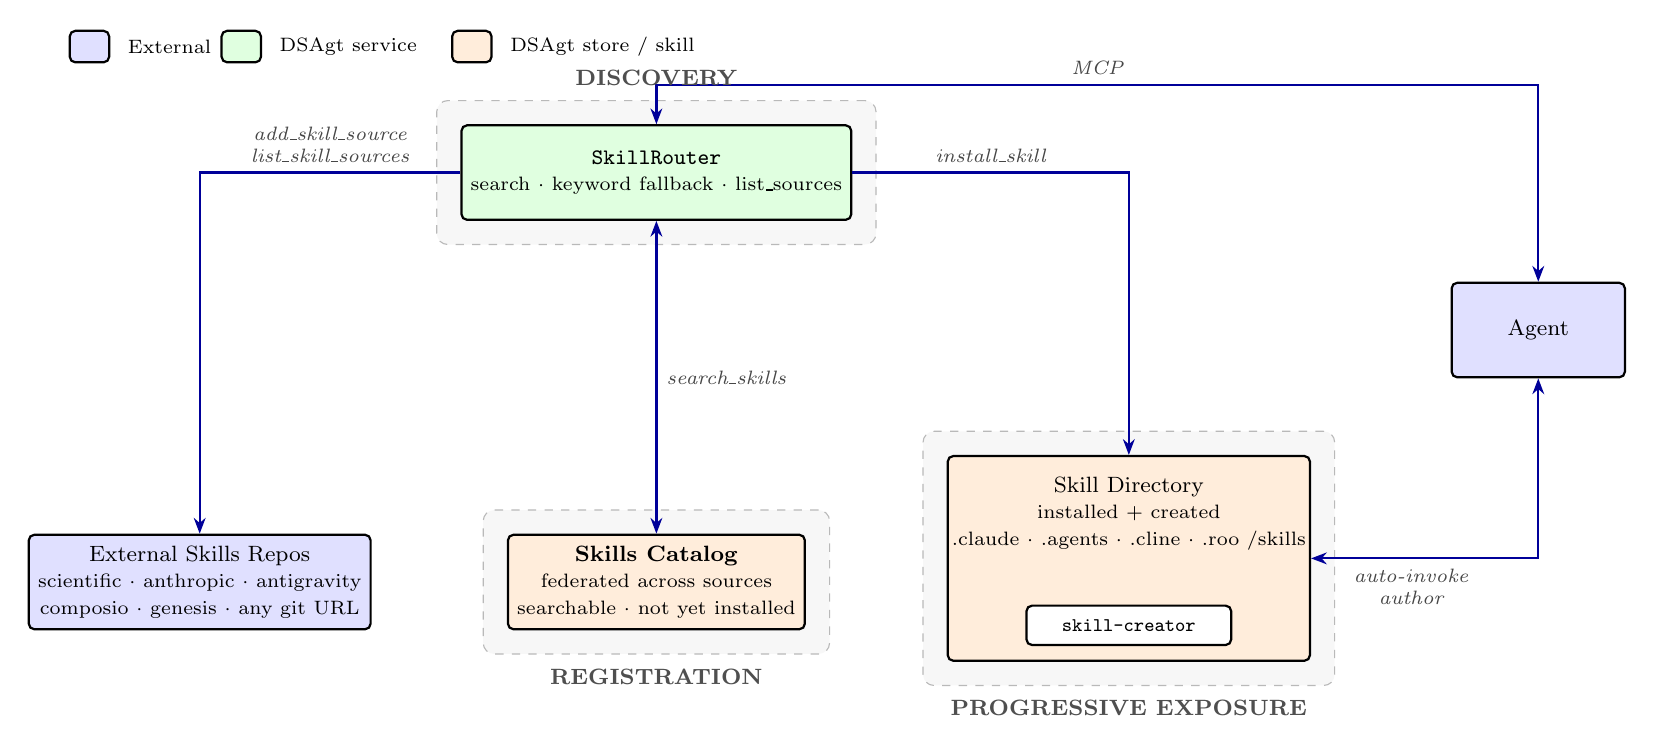
\begin{tikzpicture}[
    >={Stealth[length=2mm]},
    box/.style={
        draw, rounded corners=2pt, thick,
        minimum height=12mm, align=center,
        font=\footnotesize, fill=white},
    ext/.style={box, fill=blue!12},      % external (repos, agent)
    svc/.style={box, fill=green!12},     % DSAgt service
    store/.style={box, fill=orange!14},  % DSAgt store / skill
    skill/.style={draw, rounded corners=2pt, thick, fill=white,
                  font=\scriptsize, minimum height=5mm, align=center},
    link/.style={->, thick, blue!60!black},
    bilink/.style={<->, thick, blue!60!black},
    lbl/.style={font=\scriptsize\itshape, text=gray!55!black, align=center},
    concern/.style={font=\footnotesize\bfseries, text=gray!62!black},
    band/.style={draw=gray!55, dashed, rounded corners, fill=black!3},
]

% ============================ legend ====================================
\node[ext, minimum width=5mm, minimum height=4mm] (lk1) at (-1.6,7.4) {};
\node[right=1mm of lk1, font=\scriptsize, anchor=west] (lt1) {External};
\node[svc, minimum width=5mm, minimum height=4mm, right=14mm of lk1] (lk2) {};
\node[right=1mm of lk2, font=\scriptsize, anchor=west] {DSAgt service};
\node[store, minimum width=5mm, minimum height=4mm, right=24mm of lk2] (lk3) {};
\node[right=1mm of lk3, font=\scriptsize, anchor=west] {DSAgt store / skill};

% ============================ external (outside bands) ==================
\node[ext, minimum width=32mm] (extrepos) at (-0.2,0.6)
  {External Skills Repos\\{\scriptsize scientific $\cdot$ anthropic $\cdot$ antigravity}\\{\scriptsize composio $\cdot$ genesis $\cdot$ any git URL}};

\node[ext, minimum width=22mm] (agent) at (16.8,3.8) {Agent};

% ============================ DSAgt stores ==============================
\node[store, minimum width=34mm] (catalog) at (5.6,0.6)
  {\textbf{Skills Catalog}\\{\scriptsize federated across sources}\\{\scriptsize searchable $\cdot$ not yet installed}};

\node[store, minimum width=46mm, minimum height=26mm] (native) at (11.6,0.9) {};
\node[anchor=north, align=center, font=\footnotesize]
  at ([yshift=-1.6mm]native.north)
  {Skill Directory\\{\scriptsize installed + created}\\{\scriptsize .claude $\cdot$ .agents $\cdot$ .cline $\cdot$ .roo /skills}};
\node[skill, minimum width=26mm, anchor=south] at ([yshift=2mm]native.south)
  {\texttt{skill-creator}};

% ============================ DSAgt service =============================
\node[svc, minimum width=42mm] (router) at (5.6,5.8)
  {\texttt{SkillRouter}\\{\scriptsize search $\cdot$ keyword fallback $\cdot$ list\_sources}};

% ============================ router operations (skill MCP tools) =======
\draw[link] (router.west) -| (extrepos.north)
  node[lbl, pos=0.25, above] {add\_skill\_source\\list\_skill\_sources};
\draw[bilink] (router.south) -- (catalog.north)
  node[lbl, pos=0.5, right] {search\_skills};
\draw[link] (router.east) -| (native.north)
  node[lbl, pos=0.25, above] {install\_skill};
\draw[bilink] (router.north) -- ++(0,0.5) -| (agent.north)
  node[lbl, pos=0.25, above] {MCP};

% ============================ agent <-> skill directory (two-way) =======
\draw[bilink] (native.east) -| (agent.south)
  node[lbl, pos=0.22, below, align=center] {auto-invoke\\author};

% ============================ concern bands =============================
\begin{scope}[on background layer]
  \node[band, fit=(catalog), inner sep=3mm] (regband) {};
  \node[band, fit=(native), inner sep=3mm] (expband) {};
  \node[band, fit=(router), inner sep=3mm] (disband) {};
\end{scope}
\node[concern] at (disband.north) [above=0.6mm] {DISCOVERY};
\node[concern] at (regband.south) [below=0.6mm] {REGISTRATION};
\node[concern] at (expband.south) [below=0.6mm] {PROGRESSIVE EXPOSURE};

\end{tikzpicture}
\end{document}
